%% Sample-Paper.tex
%% V1.0
%% Developed for Authors to create their manuscript.
%%
%% This file uses the coding defined in the LaTex template ICED-Paper.cls

\documentclass{ICED-Paper}%%%%where ICED-Paper is the template name

%The authors can define any packages after the \documentclass{ICED-Paper} command.

%\usepackage{algorithmic} for describing algorithms
%\usepackage{subfig} for getting the subfigures e.g., "Figure 1a and 1b" etc.

%The author can find the documentation of the above style file and any additional
%supporting files if required from "http://www.ctan.org"

% *** Do not adjust length that controls the trim size and margins ***

\begin{document}

%The title of the paper, names of authors, affiliations of authors, abstract
%and keywords for the paper \textbf{will be produced automatically} from the
%ConfTool conference management system, based on the data that you enter in
%the ConfTool. So, don't include those details in this document.
\iffalse
What about figure \ref{fig1}?

\begin{figure}
\centering{
\includegraphics{Fig1.eps}}% Replace "fig1" with appropriate figure file name
\caption{Figure caption here\label{fig1}}
\end{figure}

Text here.

\begin{table}
\processtable{Table title here\label{tab1}}
{\tabcolsep=2pc\begin{tabular}{|l|c|}%Number of columns has to be defined here
\hline
Table text here & Table text here\\%Table body
\hline
Table text here & Table text here\\%Table body
\hline
\end{tabular}}{Table footnote here}
\end{table}
\fi

\section{Introduction}
\iffalse
    here we have to define what is the current state of understanding this phenomenon in the context of design studies and research,
    Open Source is an example of peer production in the sense that there is distributed and not centrally controled, peer to peer basis
    p2p collaborative model, management of the collaboration process,
\fi
\subsection{The emergence of open source products}
\iffalse
In the last three decades the progressive and massive adoption of computers and the internet have opened new possibilities to collaborate in unprecendented ways.Perhaps the most intriguing and solid example of this socio-technical phenomenon is the rise of the FREE/Software movement and the open source model in the software industry.
\fi

It is well known that Free Open Source Software(FOSS) rejects the distribution of software under copyright proprietary licenses and encourages the four basic user freedoms as part of its core philosophy\cite{Freedoms}: \emph{the freedom to use, study, improve and distribute the source code}. This profound paradigm shift has challenged traditional business models and classical economics assumptions that promote intellectual property as a competitive advantage \cite{Para_shift}. Further more it has shown in practice a very different approach to product development in contrast with traditional design and engineering methodologies \cite{HowItWorks}, \cite{bazaar}.
\bigskip

Over the last three decades there has been an increasing commercial adoption of free open source software (FOSS) \cite{Adoption}, being Linux OS perhaps the most emblematic case. Some of most widely used distributions of Linux includes Android(mobilephones),Ubuntu, Debian, Fedora among other thousands of distributions\cite{}. Redhat is perhaps the most known Linux based company,  The Limux project is an example FOSS Linux in public sector \cite{Limux}, which consisted in the migration of local government software from proprietary software to FOSS.There is an extensive body of empirical research that analyzes the open source software phenomenon from different angles ranging from innovation studies\cite{HowItWorks}, to organizational \cite{ActivityTheoryOpenSource} and economic studies \cite{Economics}. Von Hippel has researched open source projects revealing a different model of work that is more collaborative, open and intensively led by users \cite{HowItWorks},\cite{hippel_4},\cite{hippel_2}.
\bigskip

Similarly there has been an increasing adoption of the FOSS philosophy and practices in the hardware domain labeled as Free Open Source Hardware (FOSH)\cite{FH}, \cite{what_OH} (see Rubows technical report on FOSH \cite{Rubow} for an overview of open hardware projects until 2008). Arduino microcontrollers and RepRap 3D printers are perhaps the most prominent products in open hardware, with not only considerable adoption, but also with considerable commercial success. Adafruits and Sparkfun are two well known vendors of open hardware projects. In the case of Adafruits it is quite well known that its founder Limor Fried, also collaborates intensively within the Open Hardware Communities \cite{Million_Dollar}. Some scholars have already shed light on the similarities and differences of FOSS and FOSH, as well as critical success factors to transfer and adopt open source in the context of tangible products, \cite{OSTangible}, \cite{OSTangibleGoods}, as well as in the context of the manufacturing domain \cite{digitalCommons}. These body of research sheds light on the similarities of FOSS and FOSH but also emphasize that the experience is not directly transferable without adaptations and domain related considerations in the context of tangible goods. There is still an ongoing debate on the potentials and limitations of transfering open source software practices and tools in the context of tangible products.
\bigskip

\subsection{Research questions}

\bigskip

Design Theory and Methodology should study with carefull attention how open source works and evolves overtime. These implies analyzing the specific theories and methodologies used in open source projects, as well as those practices transfered to the domain of tangible products. Moreover this should lead to a more detailed description on what specific theories,practices and methodologies are adopted in the open source context. To move ahead in this endeavor this research attempts to address the following questions:
\bigskip

\begin{itemize}
  \item What characterizes design and development activities in the context FOSS and FOSH?
  \item How it differs from conventional theories and methodologies in the design domain?
\end{itemize}


\section{Methodology}
\emph{Without a substantive understanding of the historically changing character of the work done in a given organization, theories of design are likely to remain too general and abstract to capture the past vestiges and the emerging possibilities of design}\cite{ExpansiveDesign}
\bigskip

This section describes the theoretical background we have used to analyzed six successful open source projects (three software and three hardware projects).We use the Activity Theory framework to study open source projects, with a specific focus on the peer-to-peer aspects of the process. Activity Theory studies human behavior in a holistic fashion, and rejects the notion of isolated individual action as a unit of analysis. The main reason to choose this framework is its convenience to study and describe human action and practices in a socio-technical system. We firstly introduce the notion of commons based peer production, followed by a brief description of what  Activity Theory is and how we have used it to study the open source projects selected, with a special focus on the peer production dimension.

\subsection{Understanding open source projects as peer production systems}
\emph{In a sense, hardware is becoming much more like software, up to the point where you actually fabricate an object,"von Hippel says. "That's why you're starting to see open source techniques in hardware. Design is largely going to shift out from manufacturers to the communities}\cite{OH_Works?}
\bigskip

There is already a wide variety of studies and testimonies about the open source paradigm, including different perspectives, schools of thought, and research approaches. Most if not all of them point and/or try to describe and explain the open source model, this is the specific and most relevant relations that make many of the open source projects successful. Perhaps the most intriguing aspect of these projects is the amount participants engaged in a particular product. The number of participants in open source projects can go from ten to thousands of persons, depending on the project/community. Most well known projects work in a very decentralized and open way and do not fit with traditional industrial paradigms. In this context it is very difficult to follow each participant action and interaction with other team members.

Authors like Eric Von Hippel \cite{hippel_2}, Benkler \cite{Benkler} and Bauwens \cite{p2pEconomy} study open source projects considering a community centered approach. In these context open source is understood as a socio-technical phenomenon consisting of key relations that includes cultural, ethical, economic, technological and societal aspects, as part ot their unit of analysis. These group of authors stress the notion of peer to peer based collaboration as a key element to understand this phenomenon. While Von Hippel calls it \emph{free user to user assistance}, Bauwens calls it peer to peer and Benkler refers to it as Commons Based Peer Production(CBPP). These authors emphasize a holistic approach to this phenomenon. They give particular attention to the conditions(social, economic, technological,cultural, etc) in which these models work, succeed and evolve. Based on this research approach, this project focuses on the peer production aspects of open source projects and how the influence their progress, development and outcomes.
\bigskip

For the purposes of this work, and based on the research done by these authors, we will adopt the \emph{commons based peer production(CBPP)} term. We also adopt the a general characterization of CBPP Activity Systems according to Bawuens \cite{p2pEconomy}:

\emph{P2P specifically designates those processes that aim to increase the most widespread participation by equipotential participants. We will define these terms when we examine the characteristics of P2P processes, but here are the most general and important characteristics.
P2P processes:}

\begin{itemize}
  \item \emph{produce use-value through the free cooperation of producers who have access to distributed capital: this is the P2P production mode, a 'third mode of production' different from for-profit or public production by state-owned enterprises. Its product is not exchange value for market, but use-value for a community of users.}
  \item \emph{are governed by the community of producers themselves, and not by market allocation or corporate hierarchy: this is the P2P governance mode, or 'third mode of governance.'}
  \item \emph{make use-value freely accessible on a universal basis, through new common property regimes. This is its distribution or 'peer property mode': a 'third mode of ownership,'different from private property or public (state) property.}
\end{itemize}

\subsubsection{Using Activity Theory to understand how CBPP operates in open source projects}
In this work we used the Activity Modeling methodology developed by Larry Constantine to analyze and characterize in detail commons based peer production in the context of open source projects\cite{Constantine}. For a more in depth understanding of AT see \emph{Activity Theory in a Nutshell} \cite{ATnuthsell}.One of essential concepts of AT is that human action(individual and collective) are always oriented towards an \textbf{object}, and are mediated by \textbf{tools} in a social context(\textbf{community}).For instance a product development activity is always oriented towards a particular product, be it an Operating System, a 3D printer, or a microcontroller like Arduino. These activities are mediated by specific tools and artifacts including internalized knowledge about electronics, but also external artifacts such as as oscilloscopes, breadboards or a pencil and paper.

\begin{figure}
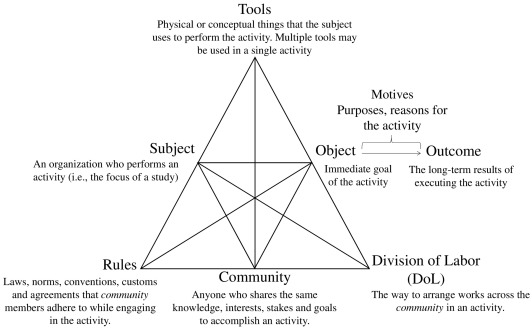
\includegraphics[width=\linewidth,height=\textheight,keepaspectratio]{AT.jpg}
\caption{\label{fig1}The figure shows the main components of AT enriched by Engestrom\cite{}. The arrows between each components express that each element in the diagram is shaped by the other elements.}
\end{figure}
\bigskip

 These activities always take place within a social context, be it a software development team, a maker space, etc. Communities have more shared \textbf{rules}, for instance safety measurements to work on a workshop, and \textbf{division of labor} or roles; for example peer review of a CAD design file, or testing code delivered by other team members.\textbf{Outcomes} stand for the actual products and impacts produced as a result of the Activity Systems dynamics. The most important aspect of these model \textf{development}, which refers to the dialectical interdependence of these components, as part of a dynamic historical process. For instance in the case of the Git version control system (\textbf{tool}), \textbf{rules} and \textbf{division of labor} issues in the context of collaborative software development are addressed by designed, as part of the structure and design specifications of the tool. As it shall be seen in the \emph{Findings} description, activity systems evolve and transform overtime, very often confronting contradictions and limitations as part of their organic development.

\section{Results: characterizing CBPP in open source projects}
In this research we have used AT to characterize commons based peer production relations and interactions within open source projects. Each project has been modeled as an activity system giving particular attention to the structural components of the model: the activity object, the subject, tools that mediate the project, collective activities , as well as the community composition, the rules and division of labor.

\begin{figure}
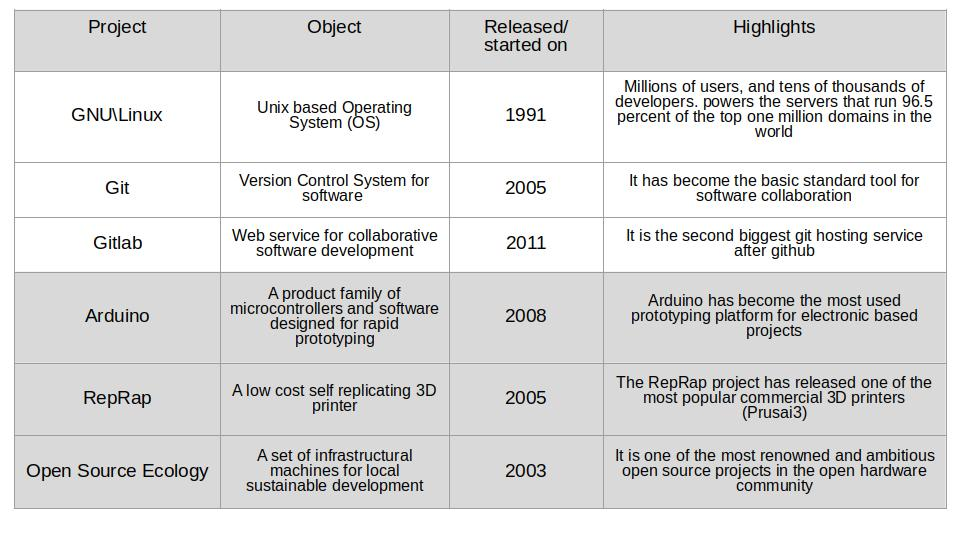
\includegraphics[width=\linewidth,height=\textheight,keepaspectratio]{Table.jpg}
\caption{\label{fig2}An overview ot the projects studied and some highlights on the impact they have made up to date.}
\end{figure}
\bigskip

\subsection{Essential artifacts in open source projects activities}
Essential artifacts that shape and develop as part of the CBPP dynamics were found in most projects. Some projects like Open Source Ecology and Gitlab were found to have less peer to peer dynamics compared to the rest of the project. Nevertheless all the projects studied present the following sets of artifacts in order to operate:
\bigskip
\begin{itemize}
\item \textbf{Regulatory artifacts}. These artifacts describe rules of the game, so to speak.Among these artifacts  find \textbf{licenses, contributing guidelines as well as code of conduct}.Licenses, for instance, address legal, ethical and commercial related aspects. It is interesting to notice that since the FREE Software licenses were created (GPL), every open source project has adopted or created similar licenses to distribute and share code, but also visual images as well as CAD files.
\item \textbf{Peer content production artifacts} There are variations in the way content creation takes place, but ultimately it requires of a web service, where other peers can access and modify the content created collaboratively. These ranges from dedicated git based services like Github, gitlab, but also wikis, forums and chats. In the case of RepRap, peer to peer interactions take place at different levels, and using different tools such as forums, and chat services within a coherence model bounded by very specific community rules.
\item \textbf{Peer review artifacts} Like peer content production, peer review relates to a more operational level within the activity system. In the case of software, version control of the code is essential. Git particularly facilitates distributed and decentralized collaboration in software projects, because it allows to do version control for highly participatory projects, and provides specific solutions for conflict management in new software releases.
\end{itemize}
\bigskip
\subsubsection{Patterns of artifacts evolution}
Artifacts (concepts, models, theories, tools, etc), develop and evolve as part of contradictions and obstacles that arise within the activity. Accommodation and re purposing existing tools from other domains is a common practice, but also extending existing tools capabilities and creating new tools. Moreover some tools embedd in their design solutions for conflict management, categorization and work organization. For instance Git solves several issues and needs that massive collaborative peer production was confronting at the time of its creation. It solved the needs and issues associated with working locally, decentralized, remotely and distributed in an integrated and effective way.
\bigskip

In some of the cases artifacts from other domains adopted in new contexts. For instance in the RepRap and Open Source Ecology, a wiki(which is also an open source system) is used to document their projects. Wikis have been originally used for peer production of written content; these open hardware communities have adopted them to share and distribute 3D models, and technical documentation. A similar case was found in Gitlab with regard to using git for version control of images and 3d models, UX designers have been struggling with new types of formats, file sizes and version control in their own domains. This contradictions have led to new extensions of Git capabilities that full fill needs such as the management of binary files, and large source code repositories. In this regard tools and objects shape each other profoundly in positive and negative ways.
\subsection{The role of users within commons based peer production}
\subsubsection{Lead innovative users}

Linus Torvalds, the creator of the Linux kernel, on an interview reveals that: \emph{Every single project I haved worked on was for something I needed.} All the open source projects studied have been developed by users that have had some level of dissatisfaction with previous solutions. These exceptional users understand very well the product they use (use-value) and commit to improve or create solutions to address their needs. What happens often is that these users are unsatisfied with the current state of a tool they use, but also with the fact that the tools shape their object in a way that is not attractive to them. In other words the products do not express the hole range of needs, values, and requirements they expect in the product/tools they used.Richard Stallman the father of the FREE/Software movement and the GNU/Linux Project, refused to accept that computer scientists, programmers and users in general were not able to study the source code.
\bigskip

Josef Prusa, a main contributor in the RepRap community explains in an interview: \emph{originally got into 3D printing because I was into music, and I started to build my own MIDI controllers. I needed all sorts of little knobs and faders. So that’s how I found 3D printing. I started to build one myself, but it took so much time and so many parts that I eventually started to make it simpler. I started to improve it and give back, and so that’s how the Prusa Simplified Mendel came to the world}.
\bigskip

There is a common motivational pattern where limitations are addressed by users and evolves towards their engagement in solving the problems they are facing, were found in the six cases studied. Also all these \emph{lead users}, have had the capacities to take hand on the solution as programmers, makers, engineers.

\subsubsection{Peer production dynamics and community composition}
Continuous peer review and feedback from other community members is perhaps the most prominent feature in most of the cases. The possibility to participate and collaborate on an equal to equal basis(peer to peer) within the community, and use the open source content without almost no restrictions, plays a very important role in community growth. It was found in different interviews and talks given by community leaders, that engaged user feedback is critical in open source projects. The RepRap forum, for instance is a common space where users share ideas, receive feedback and eventually deliver new improvements in design on a free basis. In ReRap forum was also found that some users shared solutions they have developed, and get positive response of other peers.The Arduino project also has a lot of peer to peer interactions at different levels, ranging from developers of new boards, to programmers and inventors that share their Arduino based designs and codes. In the six projects, there is an evident tendency by external peers to share ideas with different levels of engagement, but they all share publicly new ideas, comments, feedback and solutions in a very spontaneous manner.
\bigskip

Community composition also varies and segments over time, for instance new companies and entities develop reusing the open source resources, some users start new projects, or become vendors of products they have previously developed within the communities.
\subsection{Expansion of activity objects in commons based peer production}
Another important characteristic of open source projects as CBPP, is the the fact that the object is co-owned by all members of the community. On this equipotential basis. The expansion of the community composition also influences and expand the range of interests, motivations and drivers. Open source projects tend to evolve by expansion in different directions. The commercial success and focus of Linux distributions was not the main focus of Linus Torvalds (The lead engineer of the Linux Kernel), nevertheless he addresses that having the door open for other community members to join and take the project in a different direction, is a critical success factor.

\subsubsection{Integrated product extension}
It was found that some projects have evolved towards new product capabilities and integration with other products. For instance Gitlab is entirely build on the Git version control system. Third party entities and companies develop new solutions based on open source projects and also contribute considerably to open source projects.

\subsubsection{Product derivatives and variations}
At the same time, many companies and peer entities develop new variants and distribute new solutions based on available open source solutions and projects. There are literally thousands of Linux distributions, There also more than a dozen commercial RepRap 3D printer variants, distributed by different vendors. The Arduino project has also variants developed by the company and by third parties, including what they call derivatives and clones. Many of these developments take shape in a boundaryless network of peers where any entity can enrich and expand the object, but never narrow or diminish its composition.

\section{discussion}


\subsection{State of maturity of tools and infrastructures}
In contrast with software project, the tools for version control in hardware are not as advanced as in software. CAD version control and image version control is still a major issue, that influences peer to peer collaboration. The tools in software have evolve from a simple peer to peer interactions like mailing list and transfer of files, to a more integrated and enriched approach using advanced project management methodologies. The hardware projects are in a less advanced stage where the open source is released, but the collaboration workflow is not as integrated and distributed as in software.
\subsection{The influence of universal adoption in open source projects}
The possibility to collaborate in commons based peer production processes rely on being able to share and co-owned the object. In the context of computer and the internet it is scaleble and reasonable that all members of the community own a computer (means of production in this context), but this  is not necessesarily the case for complex machines like milling machines, 3D printers, cars. The specificities of the object constrain and challenge the full transfer of software practices to hardware development. Some studies have pointed out the emergence of maker spaces as a response to these limitations. But in any case, the scalability of open source projects and commons based peer production systems relies on sharing a common universal infrastructure in order to contribute and collaborate.

\subsection{Implications for design research and methodologies}
This study


\subsection{Recommendations for further studies}

\section*{References}

\bibliographystyle{unsrtnat}


  %Introduction
  \bibitem{ExpansiveDesign}Engeström, Y., 2006. Activity theory and expansive design. Theories and practice of interaction design, pp.3-23.
  \bigskip

  \bibitem{Freedoms} What is free software?, GNU, accessed 19 November 2017,
  <https://www.gnu.org/philosophy/free-sw.en.html>
  \bigskip

  \bibitem{Para_shift}Maher, M., 1999. Open source software: The success of an alternative intellectual property incentive paradigm. Fordham Intell. Prop. Media & Ent. LJ, 10, p.619.
  \bigskip

  \bibitem{HowItWorks}Lakhani, K.R. and Von Hippel, E., 2004. How open source software works:“free” user-to-user assistance. In Produktentwicklung mit virtuellen Communities (pp. 303-339). Gabler Verlag.
  \bigskip

  \bibitem{bazaar}  Demil, B. and Lecocq, X. (2006) ‘Neither Market nor Hierarchy nor Network: The Emergence of Bazaar Governance’, Organization Studies, 27(10), pp. 1447–1466. doi: 10.1177/0170840606067250.
  \bigskip

  \bibitem{Adoption}Glynn, E., Fitzgerald, B. and Exton, C., 2005, November. Commercial adoption of open source software: an empirical study. In 2005 International Symposium on Empirical Software Engineering, 2005. (p. 10). IEEE.
  \bigskip

  \bibitem{Limux} Free software in government: Munich and LiMux 2017, Free Software Foundation, accessed 19 November 2017, <https://www.fsf.org/bulletin/2017/fall/free-software-in-government-munich-and-limux>
  \bigskip

  \bibitem{ActivityTheoryOpenSource}Hemetsberger, A. and Reinhardt, C., 2009. Collective development in open-source communities: An activity theoretical perspective on successful online collaboration. Organization studies, 30(9), pp.987-1008.
  \bigskip

  \bibitem{Economics}Lerner, J. and Tirole, J., 2005. The economics of technology sharing: Open source and beyond. Journal of Economic Perspectives, 19(2), pp.99-120.
  \bigskip

  \bibitem{hippel_4}Baldwin, C. and Von Hippel, E., 2011. Modeling a paradigm shift: From producer innovation to user and open collaborative innovation. Organization Science, 22(6), pp.1399-1417.
  \bigskip

  %cited
  \bibitem{hippel_2}Von Hippel, Eric. "Democratizing innovation: The evolving phenomenon of user innovation." Journal für Betriebswirtschaft 55, no. 1 (2005): 63-78.
  \bigskip

  \bibitem{FH}Free Hardware and Free Hardware Designs 2015, Richard Stallman, accessed 19 November 2018, <https://www.gnu.org/philosophy/free-hardware-designs.en.html>
  \bigskip

  \bibitem{Rubow}Rubow, E., 2008. Open source hardware. Technical report.
  \bigskip

  \bibitem{what_OH} What is open hardware?,  opensource.com, accessed 19 November 2018,<https://opensource.com/resources/what-open-hardware>
  \bigskip

  \bibitem{Million_Dollar}Torrone, P. and Fried, L., 2010. Million Dollar Baby. Businesses Designing and Selling Open Source Hardware, Making Millions. Talk at the O'Reilly foo camp east, 1.
  \bigskip

  \bibitem{OSTangible}Raasch, C., Herstatt, C. and Balka, K., 2009. On the open design of tangible goods. R&d Management, 39(4), pp.382-393.
  \bigskip

  \bibitem{OSTangibleGoods}Balka, K., Raasch, C. and Herstatt, C., 2009, April. Open source beyond software: An empirical investigation of the open design phenomenon. In R&D Management Conference (pp. 14-16).
  \bigskip

  \bibitem{digitalCommons}Kostakis, Vasilis, Kostas Latoufis, Minas Liarokapis, and Michel Bauwens. "The convergence of digital commons with local manufacturing from a degrowth perspective: two illustrative cases." Journal of Cleaner Production (2016).
  \bigskip

  \bibitem{OH_Works?}Thompson, C., 2011. Build it. share it. profit. Can open source hardware work. Work, 10(08).

  \bigskip
  \bibitem{Benkler}Benkler, Yochai. "Peer production and cooperation." Handbook on the Economics of the Internet 91 (2016).
  \bigskip

  \bibitem{p2pEconomy}Bauwens, M., 2005. The political economy of peer production. CTheory, pp.12-1.

  \bibitem{Constantine}Constantine, L.L., 2009. Human activity modeling: toward a pragmatic integration of activity theory and usage-centered design. In Human-centered software engineering (pp. 27-51). Springer, London.

  \bibitem{ATnuthsell}Kaptelinin, V. and Nardi, B.A., 2006. Activity theory in a nutshell. Acting with technology: Activity Theory and interaction design, pp.29-72.

\end{thebibliography}
\section*{Acknowledgments}

Acknowledgments text here.

\appendix

\section*{Appendix}

Appendix text here.

\end{document}
